\chapter{Avaliação dos resultados do experimento}
	A entrada formada por ( giro, entrada, saida, metais) é correspondida respectivamente pelas entradas
	SW[3], SW[2], SW[1] e SW[0]. Para o estado B (entrando) acende o \ac{led} verde (LEDG[0]),
	para o estado de C (Detectou metal) acende o \ac{led} vermelho (LEDR[0]) e
	para o estado de D (Duas pessoas) acende o \ac{led} verde (LEDG[1]) e \ac{led}
	 vermelho (LEDR[1]). Assim, ao executar o
	\textit{test bench} obteve-se os resultados conforme as
	\autoref{figura:testBenchWaveMaquina} e \autoref{figura:testBenchTranscriptMaquina}.

	\begin{figure}[H]
		 \centering
		 \caption{\label{figura:testBenchWaveMaquina}\textit{Test bench Wave} do código da máquina.}
		 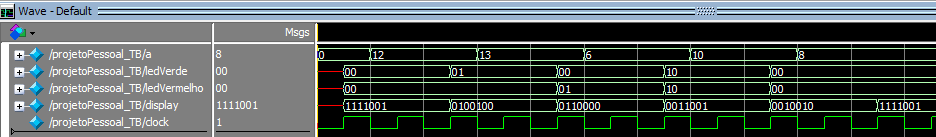
\includegraphics[width=1\textwidth]{img/wave}
	\end{figure}

	\begin{figure}[H]
		 \centering
		 \caption{\label{figura:testBenchTranscriptMaquina}\textit{Test bench Transcript} do código da máquina.}
		 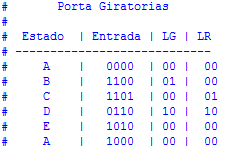
\includegraphics[width=0.5\textwidth]{img/transcript}
	\end{figure}

	Como resultado do \textit{deploy} na placa, obteve o resultado confome as
	\autoref{figura:deployMaquina1}, \autoref{figura:deployMaquina2}, \autoref{figura:deployMaquina3},
	\autoref{figura:deployMaquina4} e \autoref{figura:deployMaquina5}.

		\begin{figure}[H]
			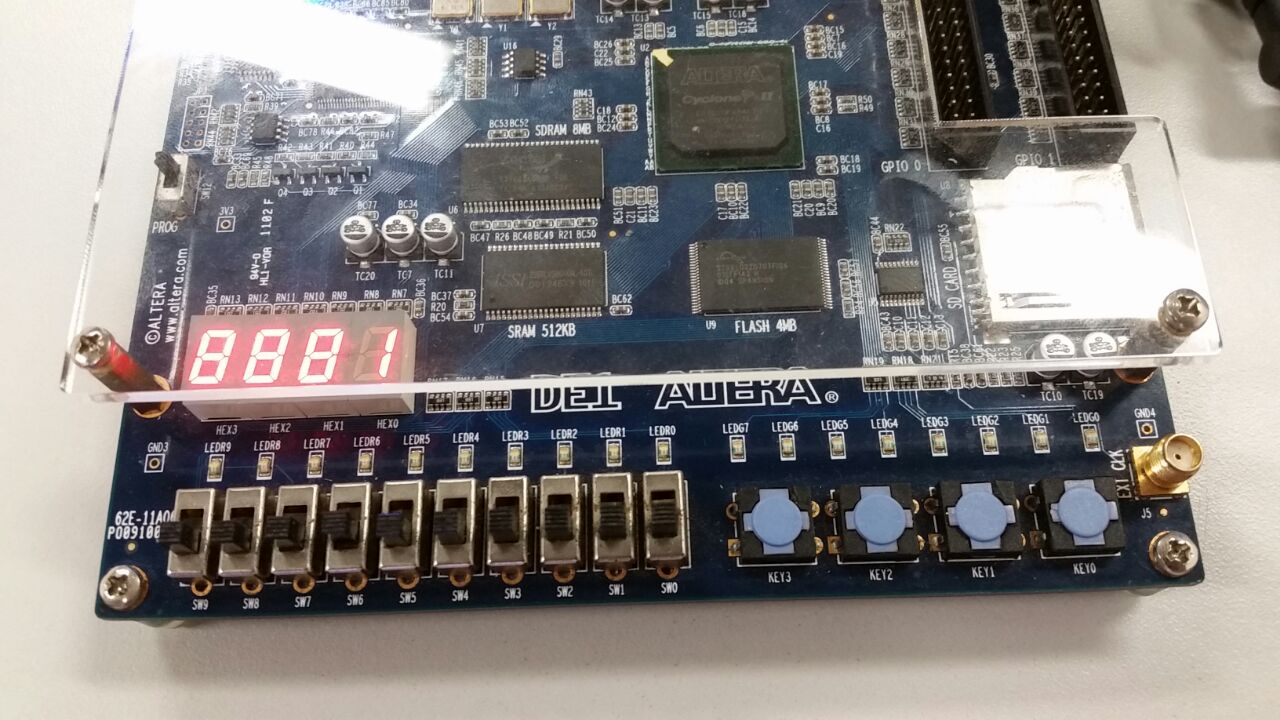
\includegraphics[width=1\textwidth]{img/placa/1}
			\caption{Máquina no estado inicial.\label{figura:deployMaquina1}}
		\end{figure}

		\begin{figure}[H]
			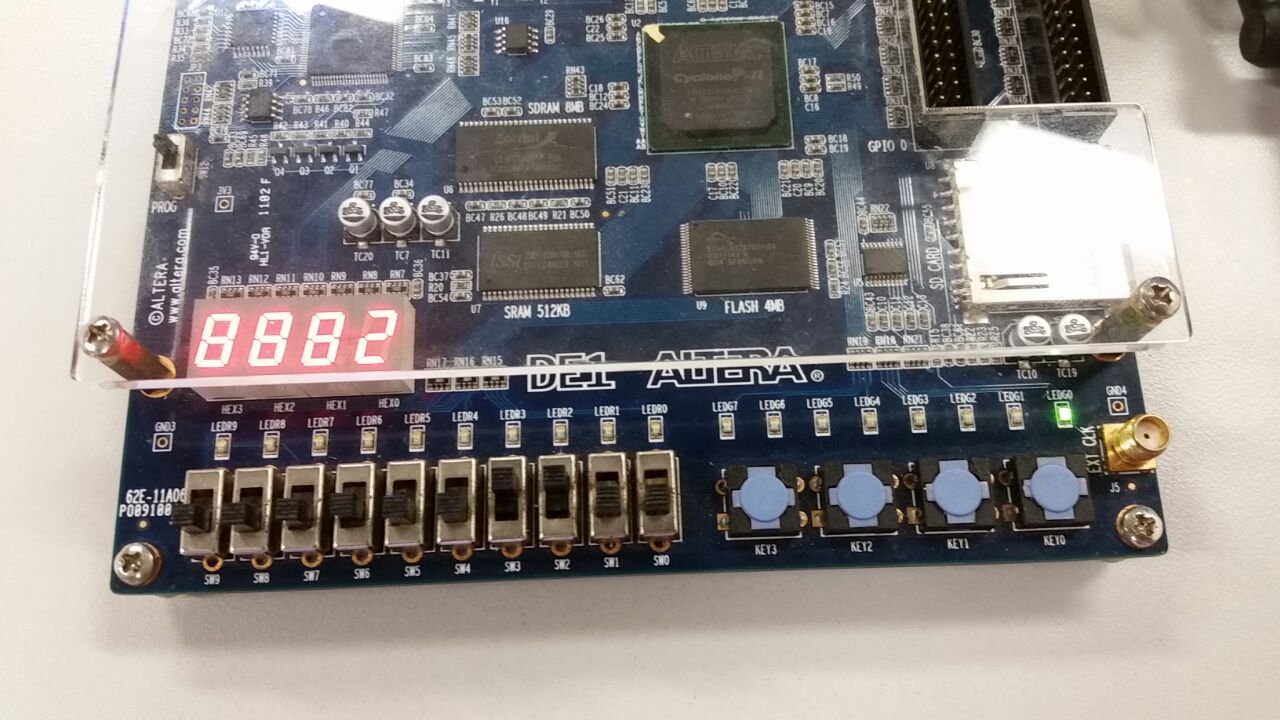
\includegraphics[width=1\textwidth]{img/placa/2}
			\caption{Transição do estado A para o B.\label{figura:deployMaquina2}}
		\end{figure}

		\begin{figure}[H]
			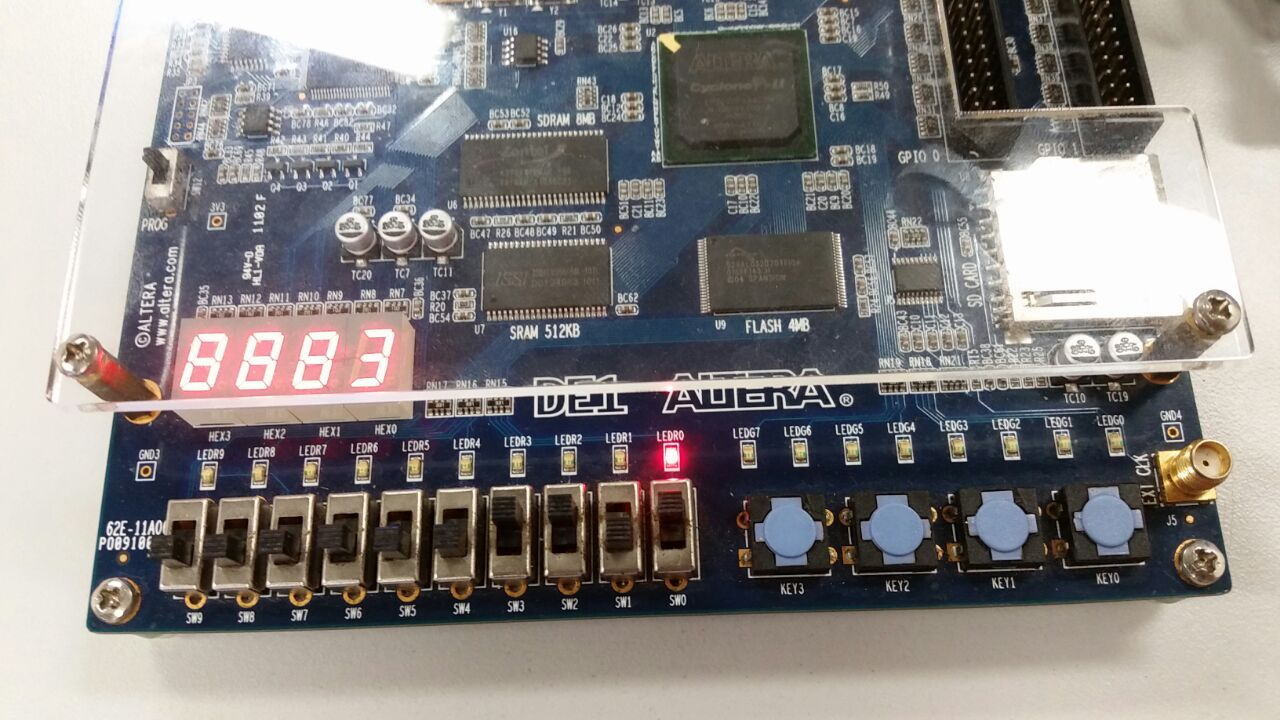
\includegraphics[width=1\textwidth]{img/placa/3}
			\caption{Transição do estado B para o C.\label{figura:deployMaquina3}}
		\end{figure}

		\begin{figure}[H]
			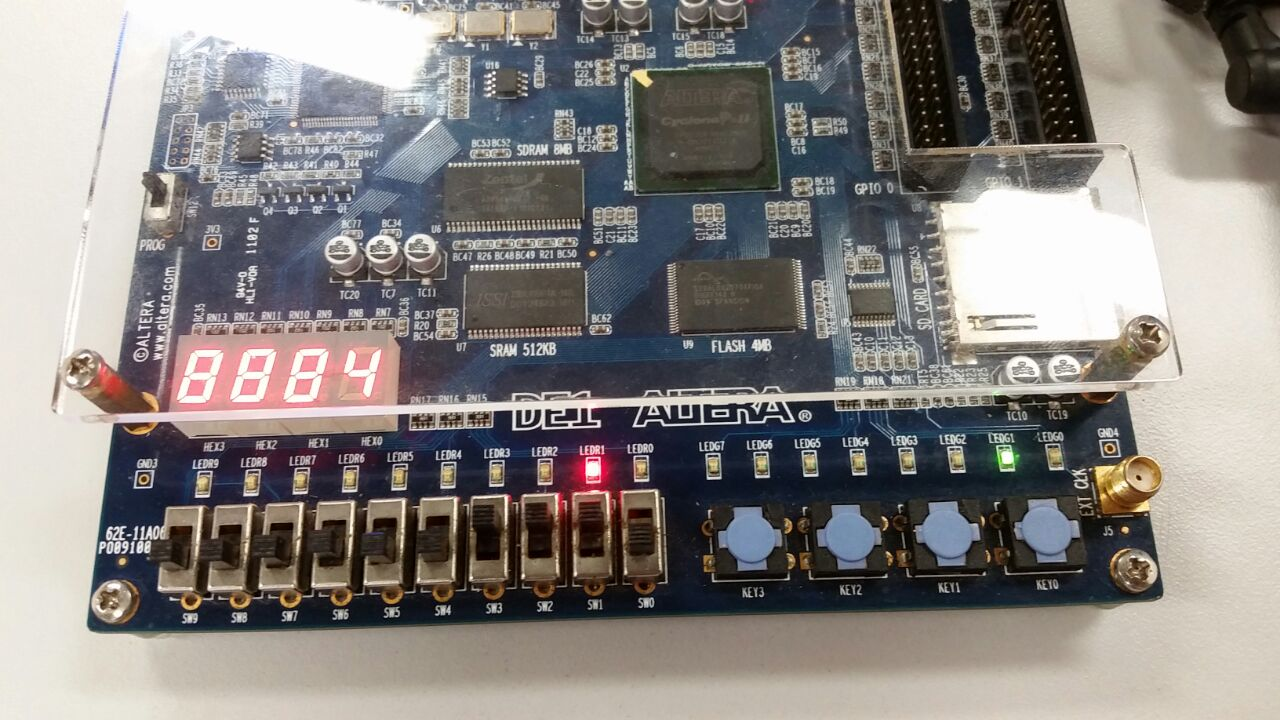
\includegraphics[width=1\textwidth]{img/placa/4}
			\caption{Transição do estado C para o D.\label{figura:deployMaquina4}}
		\end{figure}

		\begin{figure}[H]
			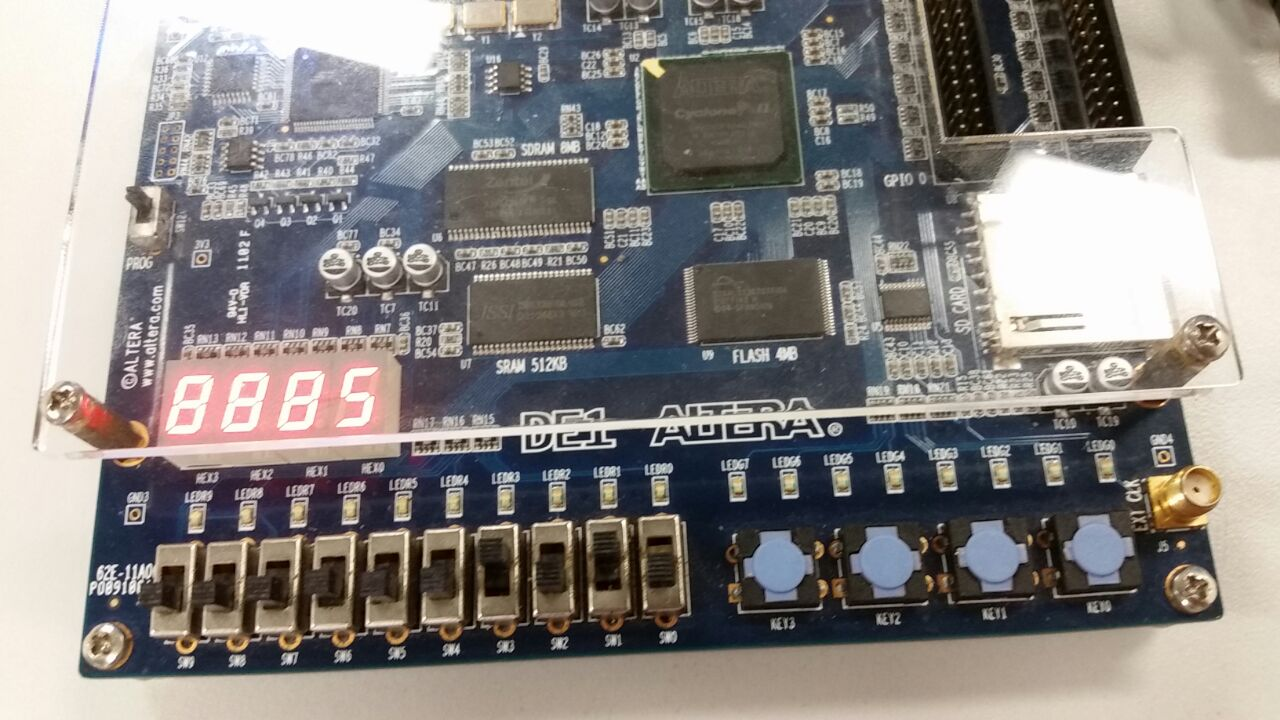
\includegraphics[width=1\textwidth]{img/placa/5}
			\caption{Transição do estado D para o E.\label{figura:deployMaquina5}}
		\end{figure}


%Apresentar os resultados da simulação em software e da utilização do Kit DE1 e/ou
%protoboard. Utilizar figuras, descrevê-las e discuti-las.
